% *** LaTeX-mal for labrapporter i FY1001 Mekanisk fysikk, NTNU ***
% Jonas Tjemsland og Rolf Jonas Persson september 2021

% Basert på LaTeX-mal for labrapporter i FY1001, v.01.11.2011, og tidligere labhefter.

% Dette er et eksempel på et LaTeX-dokument, og du kan bruke dette som et utgangspunkt for 
% din egen rapport. Den enkleste måten å komme i gang med LaTeX er ved å benytte seg
% av Overleaf (https://www.overleaf.com) gjennom en nettleser. Dette krever ingen
% installasjon og flere personer kan redigere samme dokument samtidig.

% Her i starten og videre nedover i teksten under har vi lagt inn en god del linjer som starter med
% tegnet "%". Alt som kommer etter et slikt tegn på den linja er kommentarer og vil ikke synes i den 
% ferdige teksten. Vi bruker det for å forklare ting underveis. 

% Først må vi definere noen ting for dokumentet:

% Den første linjen i ethvert TeX-dokument definerer dokumentklassen. Dette gir en overordnet stuktur
% vi bygger dokmentet på. Noen vanlige klasser er "article", "report", "book", "slides" og "letter".
% Her skal vi bruke "elsarticle", som er dokumentklassen man må bruke om man ønsker å publisere
% i Elsevier-tidsskriftene.

\documentclass[5p]{elsarticle}
% I klammeparantesen kan vi definere noen parametere som er spesifikt for hver klasse.
% For eksempel gir "5p" 2 kolonner per side, og 1p gir 1 kolonne per side. Dette er spesifikt for elsarticle.

% Vi laster inn en del pakker i starten av dokumentet som inneholder kommandoer og miløer vi vil få bruk for.
\usepackage[utf8]{inputenc}                   % Mulighet til å skrive utf8-symboler
\usepackage[norsk]{babel}				      % Tilpasning til norsk
\usepackage{graphicx}       				  % For å inkludere figurer
\usepackage{amsmath,amssymb} 				  % Ekstra matematikkfunksjoner
\usepackage[font=small,labelfont=bf]{caption} % For justering av figurtekst og tabelltekst
\usepackage{hyperref}                         % For å skrive klikkbare linker
\usepackage{float}

% Vi kan også definere egne funksjoner
\newcommand{\enhet}[1]{~\mathrm{#1}}  % Kommando for å enklere typesette enheter
\newcommand{\ve}[1]{\overrightarrow{#1}}

% Gjør noen fornorskinger (vanligvis holder et med pakken "babel", men Elsarticle ødelegger)
% Endrer fra "Preprint submitted to" til "Preprint forelagt"
\usepackage{etoolbox}
\makeatletter\patchcmd{\ps@pprintTitle}{Preprint submitted to}{Preprint forelagt}{}{}\makeatother
% Abstract -> Sammendrag
\abstracttitle{Sammendrag} % Spesifikt for elsarticle

% Her skriver man tittel og forfatterinformasjon
\title{Labrapport for semesteroppgave i FY1001 Mekanisk fysikk}
\author[fysikk]{Jacob Oliver Bruun}
\author[fysikk]{Sondre Klyve}
\address[fysikk]{Institutt for fysikk, Norges Teknisk-Naturvitenskapelige Universitet, N-7491 Trondheim, Norway.}
\journal{Labveileder} % Leveres til labveileder

%%%%%%%%%%%%%%%%%%%%%%%%%%%%%%%%%%%%%%%%%%%%%%%%%%%%%%%%%%%%%%%%%%%%%%%%%
% Selve dokumentet befinner seg i miljøet "document". Et miljø starter med kommandoen "\begin{}" og ender med "\end{}".
% Vi kommer til å benytte oss av en rekke slike miljøer i dokumentet.
\begin{document}
	
	\begin{abstract}
		Et objekts bevegelse ned en kvartsirkel kan beskrives ved ulike modeller, blant annet ved neglisjert friksjon, antatt ren rulling, og både rulling og sluring. Ved numerisk tilnærming fra Euler's metode kan slippvinkelen til objektet tilnærmes i alle disse tilfellene. Sett opp mot eksperimentelle og analytiske resultat viser det seg at den numeriske metoden utgjør en god tilnærming i å beskrive objektets bevegelse.
		
	\end{abstract}
	
	\maketitle % Denne kommanoden skriver ut dokumentinformasjonen, overskrift og sammendrag.
	
	%%%%%%%%%%%%%%%%%%%%%%%%%%%%%%%%%%%%%%%%%%%%%%%%%%%%%%%%%%%%%%%%%%%%%%%%%
	\section{Innledning}
	
	I denne rapporten brukes et oppsett hvor objekter ruller og/eller glir ned en kvartsirklet bane med ulike underlag og dermed ulik friksjon. Det vil brukes både analytiske og numeriske metoder for å regne ut vinkelen for å så teste dette mot eksperimentelle verdier. Hensikten med forsøket er å teste hvorvidt numeriske og analytiske resultater vil kunne beskrive observasjoner, og det diskuteres om resultatene er gyldige.
	
	%%%%%%%%%%%%%%%%%%%%%%%%%%%%%%%%%%%%%%%%%%%%%%%%%%%%%%%%%%%%%%%%%%%%%%%%%
	\section{Teori og metode}
	Vi ser først på et objekt med masse $m$ som glir ned en friksjonsfri halvkule med starthastighet $v_0 = 0$ og startposisjon på halvkula i en vinkel $\phi$. Vi vil da ha summen av kreftene gitt ved Newtons andre lov for translasjon, og 	ser så kun i radiell retning. Finner dermed ved sentripitalakselerasjonen
	\begin{equation}\label{sumFr}
		mg\cos(\theta) - N = ma_r = \frac{mv^2}{R+r} .
	\end{equation}
	Fra Figur \ref{figur} ser vi at vi har $h_0 = (R+r)\cos(\phi), h_1 = (R+r)\cos(\theta)$, og kan dermed ved å bruke energibevaring se
	\begin{equation}\label{vel_form}
		2mg (\cos(\phi) - \cos(\theta)) = \frac{mv^2}{R+r} .
	\end{equation}
	Kan så sette inn i likning \eqref{sumFr} og se når $N=0$ siden det er på dette tidspunktet objektet vil slippe taket på banen, og får dermed
	\begin{equation}\label{anal_løs}
	    \theta = \arccos\left[ \frac{2}{3}\cos(\phi) \right] .
	\end{equation}
	Ser videre på systemet dersom vi også inkluderer friksjon. Vi antar at den statiske friksjonskonstanten $\mu _s$ er så stor at friksjonen alltid er statisk og får dermed alltid ren rulling. Vi har fortsatt de samme argumentene som i formel \eqref{sumFr}, men pga. rulling vil vi ha et annet uttrykk for kinetisk energi. Bruker $I = cmr^2$ og $\omega ^2 = v^2 / r^2$, slik at vi ved energibevaring får
	\begin{equation}
		\frac{2mg}{1+c}\left[\cos(\phi) - \cos(\theta)\right] = \frac{mv^2}{R+r} .
	\end{equation}
	Setter så inn i likning \eqref{sumFr} med $N=0$ og får
	\begin{equation} \label{anal_rulling}
		\theta = \arccos \left[ \frac{2}{3+c}\cos(\phi) \right] .
	\end{equation}
	
	\begin{figure}[H]
	    \centering
	    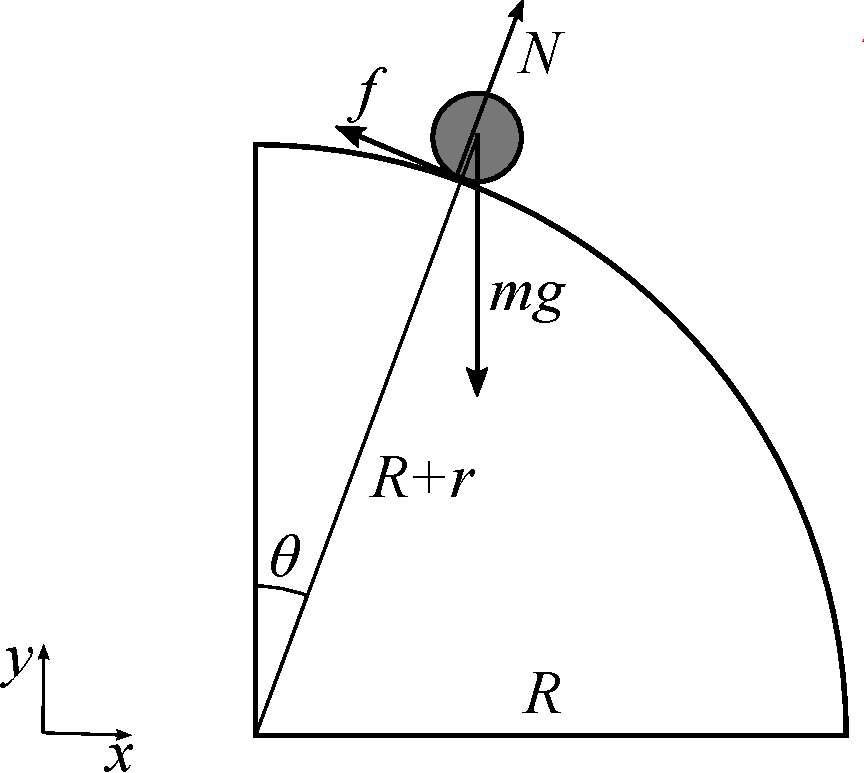
\includegraphics[width=0.3\textwidth]{figur1_good}
	    \caption{Tegning av rotasjonslegemet med krefter og størrelser}
	    \label{figur}
	\end{figure}
	
	For de numeriske løsningene brukes Eulers metode slik at
	\begin{align}
	    \theta (t + \Delta t) &= \theta (t) + \frac{d \theta (t)}{dt} \Delta t \label{euler_theta}\\
	    \omega (t + \Delta t) &= \omega (t) + \frac{d\omega (t)}{dt}\Delta t . \label{euler_omega}
	\end{align}
	Ved ren rulling har vi
	\begin{equation}\label{rrull_acc}
	    ma = mg\sin \theta - f
	\end{equation}
	og ved
	\begin{equation}
	    \alpha = \frac{\tau}{I}
	\end{equation}
	får vi $f = cma$ siden $\tau = rf$ og vi kan dermed ved å sette inn i formel \eqref{rrull_acc} få akselerasjonen som brukes for ren rulling
	\begin{equation}
	    \frac{d \omega}{dt} = \alpha = \frac{g \sin(\theta)}{1+c} .
	\end{equation}
	Ved sluring vil også formel \eqref{rrull_acc} gjelde. Kan gå fram på en likninde måte, men kan ikke anta $a = \alpha r$ slik som for ren rulling. Må derfor bruke $f = \mu_k N$. Fra likning \eqref{sumFr} har vi et uttrykk for $N$ og kan dermed bruke samme framgangsmåte, slik at vi får
	\begin{equation}
	    \frac{d \omega}{dt} = \alpha = g \sin(\theta) - \mu_k \left( g\cos(\theta) - \frac{v^2}{R + r} \right) .
	\end{equation}
	
	For å eksperimentelt finne vinkelen der objektet slipper banen, filmes bevegelsen, for å så analysere data i ``Tracker''. Det brukes forskjellige objekter, i dette tilfellet en kompakt kule, en hul sylinder og en kompakt sylinder, og de slippes uten startfart fra forskjellige startposisjoner. Det brukes et kamera (Panasonic DMC-FZ-200 med serienummer WT6EA006745), og vi valgte å filme med 100 fps (bilder i sekundet). Selv om kameraet kunne ta opp ved 200 fps valgte vi å prioritere bedre lysforhold i bildene fremfor flere bilder. Vurderingen var at dataen ville bli lettere å analysere ved få og gode bilder, fremfor flere potensielt dårligere bilder. 
	
	Kan se på usikkerhet i den analytiske metoden ved å bruke Gauss' feilforplantningslov, og får dermed
	\begin{equation}
	    \Delta \theta = \frac{2\sin (\phi)}{(c+3)\sqrt{1-\frac{4\cos ^2 (\phi)}{(c+3)^2}}} \Delta \phi
	\end{equation}
	for ren rulling, antatt at treghetsmomentet er uten feilmargin. Dette er dog en liten feil som ikke har spesiell betydning for forsøket. I tillegg er det litt vanskeligere å anslå feilmargin i den numeriske løsningen, så for å få et usikkerhetsintervall antas at alle andre størrelser enn startvinkelen er har neglisjerbare feilmarginer og det testes i ytterpunktene for å finne feilen.
	
	
	%%%%%%%%%%%%%%%%%%%%%%%%%%%%%%%%%%%%%%%%%%%%%%%%%%%%%%%%%%%%%%%%%%%%%%%%%
	
	
	\section{Resultat}
	
	%Kan se på målingene med usikkerhet fra eksperimentene i Tabell \ref{måling}. Den numeriske og analytiske unnslipningsvinkelen kan en se i Figur \ref{frikløs}. Videre kan man se på resultatene fra eksperimentene og korresponderende analytiske og numeriske utregninger for ren rulling i Tabell \ref{rrull}, og på sluring i Tabell \ref{sluring}.
	Vi vil først se på tilfellet der vi ser bort fra friksjon. Dermed vil det kun være translatorisk bevegelse nedover banen. Analytisk løsning for dette finner vi ved å sette aktuell utgangsvinkel inn i likning (\ref{anal_løs}). De numeriske dataene kommer naturligvis fra Euler's metode, altså fra (\ref{euler_theta}) og (\ref{euler_omega}). Disse resultatene kan finnes sammenliknet i figur \ref{frikløs} og tabell \ref{rfrikløs}.
	
	\begin{table}[H]
		\begin{center}
			\caption{Friksjonsløs bane, alle tall er oppgitt i grader ($^{\text{o}}$)}
			\label{rfrikløs}	% Merkelappen vi vil referere til.
			\vspace{0.5cm}					% Litt ekstra plass for å få det til å se penere ut.
			\begin{tabular}{|crr|} 		    % To venstrejusterte kolonner (l = left, c = center, r = right).
				\hline		% Horisontal linje.
				$\phi$  &  Numerisk & Analytisk\\  			% Merk symboler i kursiv, (men det er fordi de er symboler, ikke fordi de er kolonneoverskrifter!)
				\hline
				1   &  48.20  &  48.20  \\
				23  &  52.16  &  52.14  \\
				45  &  61.89  &  61.87  \\
				\hline
			\end{tabular}
		\end{center}
	\end{table}
	
	
	Videre gikk vi også eksperimentelt til verks, og gjorde en rekke målinger av utstyret vi brukte. Disse målingene brukes videre i både analystiske og numeriske utregninger. I tabell \ref{måling} er en oversikt over relevante måledata.
	\begin{table}[H]
	    \centering
	    \begin{tabular}{crr}
	        \hline
            Størrelse  &  Måling  &  Rel. usikkerhet  \\
            \hline
            $m_\text{Kule}$  &  (168 $\pm$ 1) g  &  $0.6\%$  \\
            $r_\text{Kule}$  &  (2 $\pm$ 0.5) cm  &  $25\%$  \\
            $m_\text{H. syl}$  &  (253 $\pm$ 1) g  &  $0.4\%$  \\
            $r_\text{H. syl}$  &  (4.22 $\pm$ 0.05) cm  &  $1.2\%$  \\
            $m_\text{K. syl}$  &  (896 $\pm$ 1) g  &  $0.1\%$  \\
            $r_\text{K. syl}$  &  (3.99 $\pm$ 0.05) cm  &  $1.3\%$  \\
            $R$  &  (50 $\pm$ 0.5) cm  &  $1\%$  \\
            $\phi$  &  $\pm$ 3$^{\text{o}}$ &  \\
            \hline
	    \end{tabular}
	    \caption{Målinger fra eksperimentet}
	    \label{måling}
	\end{table}
	
	Fra dette utførte vi eksperiment med ulike objekter, der målet var å oppnå ren rulling under hele bevegelsen. Dette undersøkes for både kule og kompakt sylinder, og med ulike utgangsvinkler. Tabell \ref{rrull} viser de målte verdiene, så vel som numeriske og analytiske resultat av samme situasjon.
	
	\begin{table}[H]
		\begin{center}
			\caption{Data for ren rulling, alle tall er oppgitt i grader ($^{\text{o}}$)}
			\label{rrull}	% Merkelappen vi vil referere til.
			\vspace{0.5cm}					% Litt ekstra plass for å få det til å se penere ut.
			\begin{tabular}{|crrr|} 		% Tre venstrejusterte kolonner (l = left, c = center, r = right).
				\hline		% Horisontal linje.
				$\phi$  &  Eksp. & Numerisk & Analytisk\\  			% Merk symboler i kursiv, (men det er fordi de er symboler, ikke fordi de er kolonneoverskrifter!)
				\hline \hline
				\textbf{Kule} & & & \\
				1   &  44 $\pm$ 5  &  54 $\pm$ 0.1  &  53.97 $\pm$ 0.04  \\
				23  &  60 $\pm$ 5  &  57 $\pm$ 1  &  57.2 $\pm$ 0.8   \\
				45  &  66 $\pm$ 5  &  66 $\pm$ 2  &  64.4 $\pm$ 1.3  \\
				\hline \hline
				\textbf{Sylinder} & & & \\
				2   &  49 $\pm$ 5  &  55.2 $\pm$ 0.1   &  55.17 $\pm$ 0.07  \\ 
				23  &  58 $\pm$ 5  &  58 $\pm$ 1   &  58.3 $\pm$ 0.8  \\
				44  &  64 $\pm$ 5  &  66 $\pm$ 2  &  65.7 $\pm$ 1.3  \\
				\hline
			\end{tabular}
		\end{center}
	\end{table}
	% Litt ekstra forklaring av tabellen til slutt:
	% Du skiller altså kolonnene med tegnet "&", og du setter inn linjeskift med "\\".
	% (Dersom du får problemer med at kommaene ikke flukter i kolonnen, se kap. 8.3.1 i labheftet, eller bruk f.eks. pakken siunitx.)
	% De horisontale linjene er plassert ifølge standarden du etterhvert bør ha begynt å bli vant til.
	
	% Før man har lært seg å bruke LaTeX bør man ikke prøve å tvinge dokumentet til å se ut på en spesiell måte.
	% En av de store fordelene med LaTeX er at man kan skrive teksten uten å tenke på dokumentformateringen. Denne er nemlig
	% allerede satt opp for oss! LaTeX ordner alt av sideskift og bildeplasseringer for oss og det blir som regel bra dersom man har
	% satt opp dokumentet rett.
	\begin{table}[H]
	    \begin{center}
	        \caption{Data for sluring ved aluminium mot stål. Bruker da $\mu _s = 0.5$ og $\mu _k = 0.45$ \cite{Haugan}. Alle tall er oppgitt i grader ($^{\text{o}}$)}
	        \label{metall2}
	        \begin{tabular}{|crr|}
	            \hline
				$\phi$  &  Eksp. & Numerisk  \\
				\hline \hline
				\textbf{Hul sylinder} & &  \\
				1   &  56 $\pm$ 5  &  55.45 $\pm$ 0.05   \\
				21  &  60 $\pm$ 5  &  56.5 $\pm$ 0.7   \\
				43  &  63 $\pm$ 5  &  64 $\pm$ 2    \\
				\hline \hline
				\textbf{Sylinder} & &  \\
				1   &  56 $\pm$ 5  &  53.4 $\pm$ 0.1   \\
				23  &  58 $\pm$ 5  &  56.4 $\pm$ 0.8   \\
				43  &  64 $\pm$ 5  &  63 $\pm$ 2   \\
				\hline
	        \end{tabular}
	    \end{center}
	\end{table}
	
	
	Til slutt ble det forsøkt å få objektet til å gå over til sluring underveis i bevegelsen. Altså ville vi ha ren rulling frem til et punkt der farten tvingte frem sluring. Eksperimentelt brukte vi da baner med glatt overflate for minimert friksjon, slik at objektet skulle gå over til sluring etter hvert. I denne situasjonen har vi ikke analytiske resultater, men fremdeles observerte og numeriske målinger, sett i tabell \ref{metall2} og \ref{sluring}.
	
	\begin{table}[H]
	    \begin{center}
	        \caption{Data for sluring ved aluminium mot teip. Antatt friksjonskeoffisient som stål på stål med smurte overflater, og bruker da $\mu _s = 0.1$ og $\mu _k = 0.08$ \cite{Haugan}. Alle tall er oppgitt i grader ($^{\text{o}}$)}
	        \label{sluring}
	        \begin{tabular}{|crr|}
	            \hline
				$\phi$  &  Eksp. & Numerisk  \\
				\hline \hline
				\textbf{Hul sylinder} & &  \\
				0   &  47 $\pm$ 5  &  50.3 $\pm$ 0.1   \\
				22  &  58 $\pm$ 5  &  53 $\pm$ 1   \\
				43  &  69 $\pm$ 5  &  61 $\pm$ 2    \\
				\hline \hline
				\textbf{Sylinder} & &  \\
				1   &  64 $\pm$ 5  &  50.2 $\pm$ 0.1   \\
				22  &  68 $\pm$ 5  &  53 $\pm$ 1   \\
				42  &  68 $\pm$ 5  &  61 $\pm$ 2   \\
				\hline
	        \end{tabular}
	    \end{center}
	\end{table}
	
	\section{Diskusjon}
	
	Ved antatt friksjonsfri bane er utregningen kun avhengig av utgangsvinkelen til objektet. Det betyr at formen på objektet heller ikke har noe å si. Dette er fordi vi ved null friksjon vil ha ren translatorisk bevegelse, slik at ingen rulling kan fremkomme. Resultatet blir at vi kan se helt bort i fra treghetsmomentet til det relevante objektet. Grunnet lite avhengighet i utregningene er det også rimelig å anta gode tilnærminger numerisk, noe vi fra tabell \ref{rfrikløs} ser at vi får. Med presisjonen vi har brukt i Euler's metode har vi kommet meget nærme de analytiske verdiene, noe som også er reflektert i figur \ref{frikløs}. Merk at alle disse antagelsene gjør modellen for bevegelsen svært virkelighetsfjern.
	
	\begin{figure}[H]
	    \centering
	    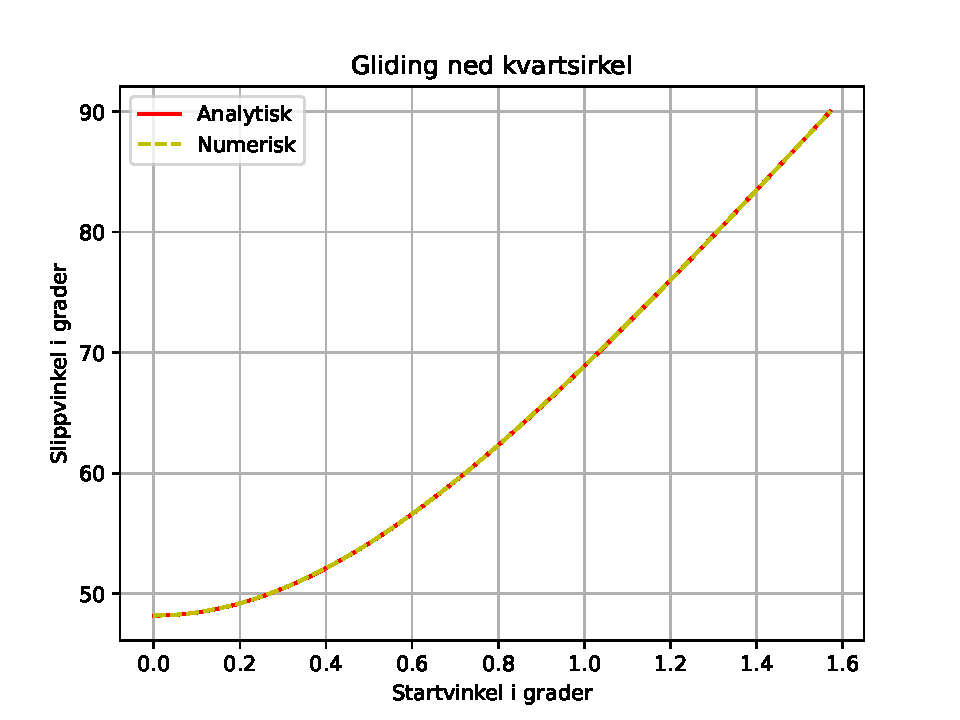
\includegraphics[width=0.5\textwidth]{Figure_0}
	    \caption{Graf med analytisk og numerisk unnslipsvinkel til sammenlikning ved friksjonsløst underlag.}
	    \label{frikløs}
	\end{figure}
	
	Fra tabell \ref{rrull} ser vi resultatene fra forsøket ved ren rulling. I eksperimentet brukte vi en bane med overflate i filt, slik at friksjonen skulle være størst mulig. Ved stor friksjon vil objektet oppnå ren rulling gjennom hele bevegelsen. Tilsvarende som ved null friksjon stemmer de numeriske og analytiske verdiene ganske godt, og danner et grunnlag for hva vi kunne forvente oss fra observerte målinger. Som vi kan se, er ikke de observerte målingene like fint i tråd med resten av målingne, men følger i det minste en tilsvarende trend. Dette skyldes nok heller feilmargin i observasjon enn feil i numerisk eller analytisk løsning.
	
	%Ser at for friksjonsløst underlag er den numeriske og den analytiske unnslipningsvinkelen omtrent den samme. I tillegg stemmer de numeriske løsningene fra koden overens med den analytiske løsningen når en ser på ren rulling også. De eksperimentelle målingene for den kompakte sylinderen stemmer ganske godt med numerisk og analytisk løsning for de to slippunktene som ikke er helt øverst på banen. De eksperimentelle resultatene for kula er derimot usedvanlige da kula slipper senere for et høyere slippunkt, noe som går mot den analytiske løsningen som vist i  \eqref{anal_rulling}. Vi kan derfor ikke stole fullt på disse målingene.
	
	Ved å bruke en baneoverflate dekket av teip og en bane i stål kan en håpe på å oppnå at objektet vil rulle rent først, og etter hvert, ved en tilstrekkelig fart, gå over i sluring. Fra tabell \ref{metall2} og tabell \ref{sluring} har vi målinger gjort eksperimentelt, samt en numerisk estimasjon av forsøket. I dette tilfellet har vi altså ikke noen analytisk løsning på problemet. Kun sylindere ble tatt i betraktning, og kan i resultatet se at store deler av observasjonene ikke stemmer helt overens med den numeriske løsningen. Dette har nok mye å gjøre med at det var vanskelig å avgjøre den nøyaktige vinkelen sylindere slipper banen ved videoanalyse. Det fører til en stor feilmargin som kan forklare spriket i dataen.
	
	Dersom en ser på sluring med forskjellige overflater, se tabell \ref{metall2} og tabell \ref{sluring}, så kan en se at ifølge de numeriske dataene og resonnementen som ble gitt tidligere burde objektene slippe taket til banen senere når friksjonskoeffisienten er større. Dette gjenspeiles kun i to av resultatene i disse tabellene. Dette kan komme av den store feilmarginen som vises i den eksperimentelle målingen av unnslipsvinkel, men likevel ser en at det så vidt er overlapp i det estimerte intervallet i en kompakt sylinder som blir sluppet ved ca. 22$^{\text{o}}$. Dette viser også at det finnes store feil i den eksperimentelle dataen, da det i teorien skal være mer slik som numerikken viser. En annen feilkilde i dette tilfellet kan være friksjonskoeffisientene, og at teip mot aluminium har større friksjonskoeffisient enn smurt stål mot stål, men som en ser senere så finnes det ingen $\mu_s, \mu_k$ som oppfyller den eksperimentelle dataen i tabell \ref{sluring}.
	
	En fellesnemner i måledataene våre er at de observerte målingene tenderer til å avvike fra de analytiske og numeriske estimatene. Dette skyldes i hovedsak vanskelighet rundt å avgjøre nøyaktig når objektet slipper banen. I tilfellet med kulen vil det være spesielt utfordrende, da kulen er senket i sporet på banen. Utover det gjorde vi et valg i vinklingen av kameraet der vi ville filme mest mulig rett på. Det førte til gode målinger undervegs, men gjorde det altså vanskelig å avgjøre slippvinkelen nøyatkig. En annen faktor som spiller inn, og som spesielt målingene i tabell \ref{metall2} og \ref{sluring} bærer preg av, er uklarhet i bildet ved høy hastighet på objektet. Som tidligere diskutert spørs det om høyere bildefrekvens i videoen ville vært til nytte i dette tilfellet. Antagelig ville det spilt en liten rolle i den allerede betydelige usikkerheten rundt observerte målinger. Det en kan trekke ut av dette er at kodens kredibilitet ikke nødvendigvis burde bli svekket grunnet sprik i data, men at dette heller skyldes unøyaktige observasjoner fra eksperimentet.
	
	Fra tabell \ref{måling} ser vi at radiusen til kula har en voldsom feilmargin. Dette skyldes utformingen av banen, som dannet et spor kula lå i. Siden kula var senket i dette sporet vil ikke den målte radiusen av kula stemme overens med resten av våre antagelser. Dette er forsøkt korrigert ved å anta at kula senket i sporet utgjør en bevegelse tilsvarende den av en mindre kule som ligger fullstendig på banen, altså en kule som ikke faller ned i noe spor. Dette forklarer hvorfor den relative usikkerheten til kulas radius er så stor.
	
	%Ser likevel at de andre eksperimentelle resultatene også er ganske forskjellig fra hva den numeriske unnslipsvinkelen skulle tilsi. En kan derfor spørre seg om det er numerikken eller om det er eksperimentene som står for mesteparten av feilene? Som tidligere nevnt, og som en ser i Figur \ref{frikløs}, er det meget liten, om noen, forskjell i den analytiske og den numeriske unnslipningsvinkelen for ingen friksjon. En kan også se i Tabell \ref{rrull} at den numeriske løsningen er ganske lik den analytiske, og siden koden for oppgave 3 er bygget på koden fra de to foregående løsningene, vil en tro at det sannsynligvis ikke er en feil i koden. En kan også se på ytterpunkter i koden for tredje problem, og teste den opp mot situasjoner vi kjenner analytiske løsninger til. Ved å for eksempel sette $mu_s, mu_k = 0$, vil man få en friksjonsløs gliding. Svaret som koden fra oppgave 3 gir, stemmer overens med den analytiske løsningen som er utarbeidet i Formel \eqref{anal_løs}. Man kan også sette $\mu _s$ stor nok til å få utelukkende ren rulling. Også her vil koden i oppgave 3 korrespondere med den analytiske løsningen i Formel \eqref{anal_rulling}.
	
	En interessant observasjon en kan gjøre ved å analysere data fra den numeriske løsningen, er at akselerasjonen har et hopp, som vist i Figur \ref{acc}. Dette skjer når objektet går over fra ren rulling til sluring. Selv om dette ser veldig unaturlig ut, kan det forklares ved at akselerasjonen går fra å være avhengig av den statiske friskjonskoeffisienten, $\mu_s$, til å være avhengig av den kinetiske friksjonskoeffisienten, $\mu_k$. Siden $\mu_s > \mu_k$ vil friksjonskraften plutselig bli mindre fordi den går fra $f \leq \mu_s N$ til $f = \mu_k N$. Det er kun akselerasjonen som oppfører seg slikt, farten kan få et knekkpunkt i dette punktet, men vil ikke hoppe slik som akselerasjonen.
	
	\begin{figure}[H]
	    \centering
	    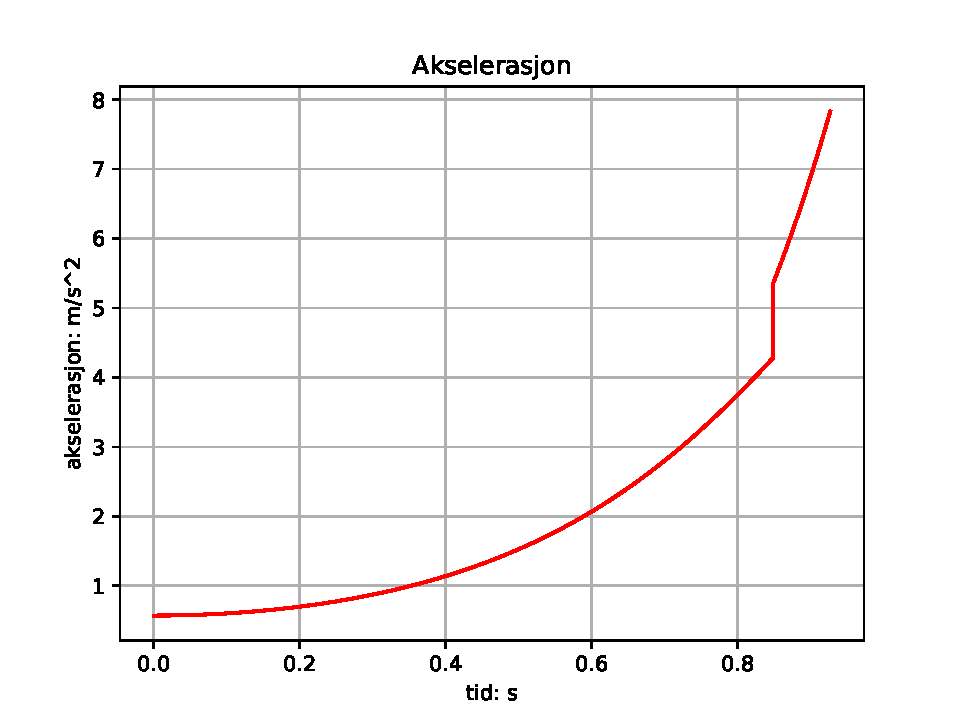
\includegraphics[width=0.5\textwidth]{Figure_acc}
	    \caption{Akselerasjon i for en kompakt sylinder med $\mu_s = 0.5, \mu_k = 0.25$}
	    \label{acc}
	\end{figure}
	
	Et resultat av måten vi har skrevet koden, er at resultatet for slippvinkelen alltid vil falle i et gitt intervall; nemlig mellom ingen friksjon og ren rullling. Ved null friksjon vil det ikke vere noen kraft som virker mot den translatoriske bevegelsen. Dermed vil akselerasjonen være på sitt største, og objektet vil slippe banen tidlig. Motsatt vil ren rulling gjøre all friksjon om til rulling, som bremser den translatoriske akselerasjonen, og gjør at objektet slipper senere. Siden noen av observasjonene våre faller utenfor dette intervallet, vil ikke koden kunne treffe den eksperimentelle dataen. Dette er spesielt aktuelt i oppgave 3, der vi ser på en blanding mellom rulling og sluring. 
	
	%Dersom en justerer $\mu_s$ og $\mu_k$ for den kompakte sylinderen i koden, vil ikke de samme resultatene som de eksperimentelle oppstå. Dette kommer av at den numeriske løsningen alltid vil ha en øvre grense som er når det er ren rulling, og for den kompakte sylinderen er de eksperimentelle avleste dataene større en unnslipsvinkelen når det er ren rulling. At numerikken ved sluring ikke tillater en unnslipsvinkel større enn den for ren rulling taler også for koden, siden akselerasjonen alltid vil bli større når objektet går over til sluring og den vil dermed slippe tidligere. En kan også se resultatene i Tabell \ref{rrull} og Tabell \ref{sluring}. Den numeriske løsningen viser at sylinderen skal slippe senere ved ren rulling, men i eksperimentet ser en at dette ikke stemmer.
	
	\begin{figure}[H]
	    \centering
	    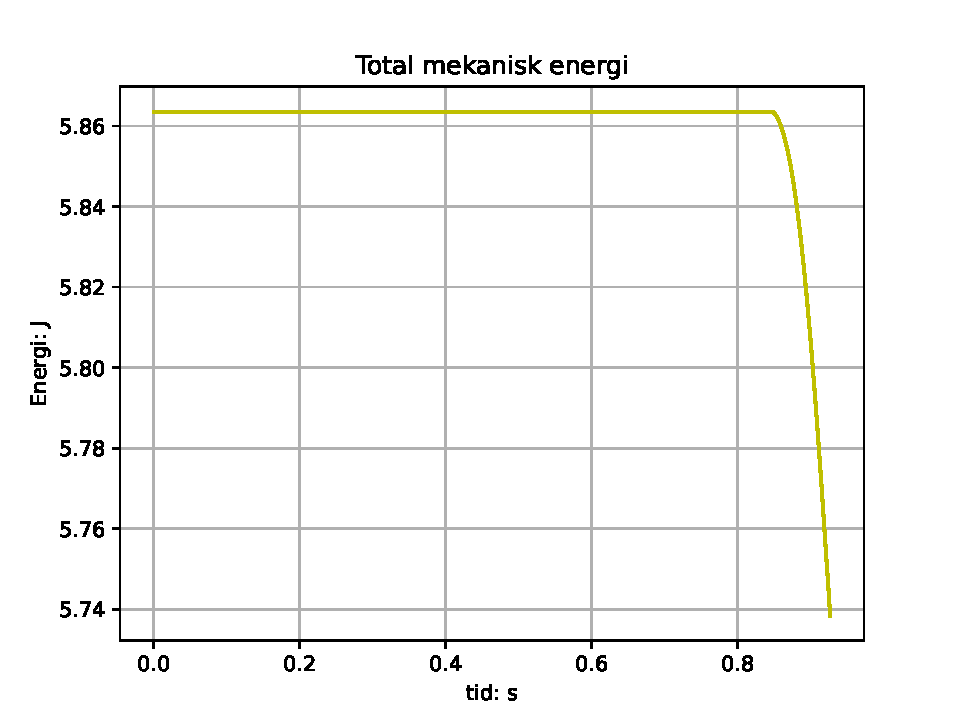
\includegraphics[width=0.5\textwidth]{Figure_e}
	    \caption{Mekanisk energi for kompakt sylinder med $\mu_s = 0.5, \mu_k = 0.25, m = 1\enhet{kg}$}
	    \label{energy}
	\end{figure}
	
	I figur \ref{energy} kan vi se at den mekaniske energien i systemet er bevart frem til objektet begynner å slure. Siden bevegelsen frem til dette punktet består av ren rulling, vil det kun være konservative krefter som virker, og den mekaniske energien skal dermed være bevart \cite{Lien}. Vi kan dermed konkludere med at resultatet fra koden stemmer godt overens med det man skulle  anta teoretisk sett. Likevel vil en oppdage at dersom en zoomer inn mye på den mekaniske energien vil en se at det ikke er en rett linje, men at den veldig sakte bøyer seg ned. Dette kommer sannsynligvis av at Eulers metode blir brukt, både for å finne hastigheten til objektet og for å finne vinkelhastigheten i legemet under sluring. Kan se at forskjellene er så små at selv ved bruk av liten $\Delta t$ vil det være en liten feil, men denne er så ubetydelig at en kan se bort fra den.
	
% 	\begin{figure}[H]
% 	    \centering
% 	    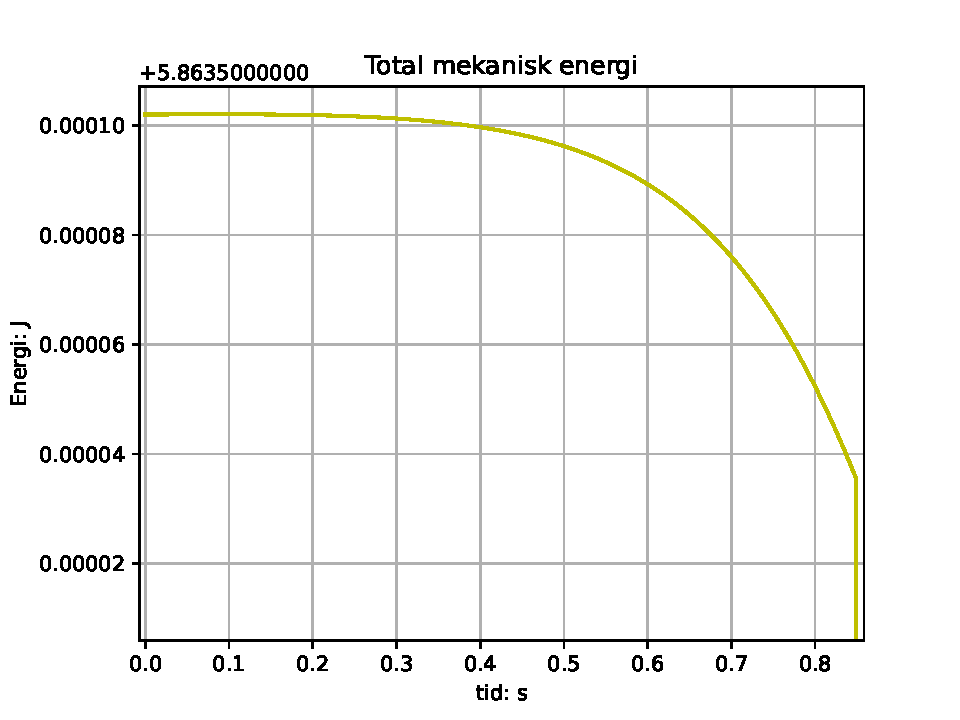
\includegraphics[width=0.5\textwidth]{Figure_ez.pdf}
% 	    \caption{Mekanisk energi for kompakt sylinder med $\mu_s = 0.5, \mu_k = 0.25, m = 1 \enhet{kg}$}
% 	    \label{Ezoom}
% 	\end{figure}
	
	%Kan også se at den mekaniske energien er bevart frem til punktet hvor objektet går over til sluring, dette gir mening da det fram til dette punktet er kun konservative krefter som virker. Dette er enda et punkt som gir tiltro til den numeriske koden framfor de eksperimentelle resultatene.
	
	
	%%%%%%%%%%%%%%%%%%%%%%%%%%%%%%%%%%%%%%%%%%%%%%%%%%%%%%%%%%%%%%%%%%%%%%%%%
	\section{Konklusjon}
	Vi har sett at en numerisk tilnærming av forsøket ved Euler's metode gir veldig gode resultat sett opp mot analytiske løsninger på problemet. Videre har vi sett at der det ikke er utarbeidet noen analytisk løsning, har den eksperimentelle og numeriske løsningen hatt noe avvik, men fremdeles fulgt en lignende utvikling med hensyn på friksjon og utgangsvinkel. Eventuelle avvik mellom numeriske og observerte målinger ser ut til å i stor grad skyldes unøyaktighet i målingene. Basert på alle situasjoner vi da har tatt for oss i rapporten, kan vi konkludere med at den numeriske løsningen gir en god beskrivelse av forsøket.
	%\textit{
		%Konklusjonen er rapportens viktigste del. I konklusjonen legger du frem ditt egentlige faglige bidrag. Det er som regel formidlingen av dette bidraget som er hovedgrunnen til at du skriver rapporten. Konklusjonskapitlet bør ikke skrives før du har tenkt grundig over resultatene fra dine egne målinger og sammenlignbare målinger gjort av andre i lys av den teori du har valgt å tolke resultatene innenfor. En god konklusjon er kort og presis, og presenterer kun hovedresultatet og konklusjonen fra diskusjonen. Eventuelt fremtidig arbeid kan også nevnes her. 
	%}
	
	%%%%%%%%%%%%%%%%%%%%%%%%%%%%%%%%%%%%%%%%%%%%%%%%%%%%%%%%%%%%%%%%%%%%%%%%%
	
	% Her kommer referanselisten. Dersom du ønsker flere enn noen få referanser, kan det lønne seg å 
	% søke opp "BibTeX" og sette seg litt inn i det. 
	\begin{thebibliography}{99}	% Denne referanselisten kan ikke ha flere enn 99 referanser.
		
		\bibitem{Haugan} 
		J. Haugan og E. Aamot. \textit{Gyldendals tabeller og formler i fysikk}. Gyldendal Norsk Forlag AS, 2. utgave, 2011.
		
		\bibitem{Lien} % I klammeparentes angir vi merkelapp for de ulike oppføringene i listen.
		J. R. Lien og G. Løvhøiden. \textit{Generell fysikk for universiteter og høgskoler}, bind 1. Universitetsforlaget, 3. opplag, 2010.
		
	\end{thebibliography}
	
\end{document}
